\chapter{rComplexity in Practice}

\section{Human-driven calculus of rComplexity}
This section aims to present a simple methodology of calculating by hand the associated rComplexity class for any given algorithm, provided a predefined instruction set architecture and the correspondence between generic instructions and required time for execution as well as enhanced hardware designs details related to the total execution time (no. of stages of pipeline, scalability degree, etc.). Even if the process of calculating an exact rComplexity class associated to a real algorithm is unpractical, the method provided can be applied with colossal endeavor. Later on, we will present an automated method of estimating the rComplexity of a given algorithm.

\subsection{N-Queens’ Problem}
We will begin to solve this by making an observation about choosing the $N$ Queens on the board with the dimensions $n$ x $n$. In order not to have attacks between two Queens, it must not have two Queens on the same line or column. We define a Queen $Q$ by the pair on points $ (x, y) $, where $ x, y \leq n $, are the coordinates corresponding to the position on the chessboard.
The problem can be solved by checking all possible permutations: $ Q (1) = (1, y_1) $ , 
$ Q (2) = (2, y_2) $ ... , $ Q (n) = (n, y_n) $ \\
where $ y_1, y_2, ..., y_n \ in \ { 1,2, ..., n \ } $ and $ y_1, y_2, ..., y_n $ distinct. In these conditions, the only action that still needs to be verified is that of the "diagonal attack" of Queens.

\begin{algorithm}[H]
\caption{Exhaustive N-Queens’ Problem Pseudocode}
\begin{algorithmic}[1]
\Procedure{QueenProblem}{$currentMatrix,row,column$}
\If {$column=1$ and $row=n+1$}
	\State print currentMatrix
	\State Return

\EndIf
\For {i=1..n}
	\If {noConflict(currentMatrix,row,column) = TRUE}
		\State $currentMatrix[row][i] \gets 1$
		\State $QueenProblem(currentMatrix,row+1,1)$
		\State $currentMatrix[row][i] \gets 0$
		//BackTracking Step
	\EndIf
\EndFor
\EndProcedure
\Procedure{Main}{$n$}

\State $read\ n$
\State $currentMatrix.initiate()$
\State $currentMatrix.setrows(n)$
\State $currentMatrix.setcolumns(n)$
\State $currentMatrix \gets$
$\left[\begin{array}{ccccc}
0 & 0 & ... & 0 & 0	\\
0 & 0 & ... & 0 & 0	\\
 &  & ... &  & 	\\
0 & 0 & ... & 0 & 0	\\
0 & 0 & ... & 0 & 0	\\
\end{array}\right]$ 
\State $QueenProblem(currentMatrix,1,1)$
\EndProcedure
\end{algorithmic}
\end{algorithm}

\begin{algorithm}[H]
\caption{noConflict Helper function}
\begin{algorithmic}[1]
\Procedure{noConflict}{$currentMatrix,row,column$}
	\For {i=1..row-1}
		\If {currentMatrix[i][column] = 1}
			\State \Return FALSE
		\EndIf
	\EndFor
	
	
	//Check on "diagonal" parallel with second diagonal
	\State $i \gets row$
	\For {j=column..n}
	\If {currentMatrix[i][j] = 1}
			\State \Return FALSE
		\EndIf
	\If {$i \leq 0$}
		\State break
	\EndIf
	\State $i \gets i-1$	
	\EndFor
	
	//Check on "diagonal" parallel with main diagonal
	\State $i \gets row$
	\For {j=column..0 : increment -1}
	\If {currentMatrix[i][j] = 1}
			\State \Return FALSE
		\EndIf
	\If {$i \leq 0$}
		\State break
	\EndIf
	\State $i \gets i-1$	
	\EndFor

\EndProcedure

\end{algorithmic}
\end{algorithm}

To begin with, here is a method of calculating traditional complexity using the classical model.
To calculate the complexity of the QueenProblem algorithm, we will individually analyze the complexities of the operations in the QueenProblem function. We will note with $n$ the number of Queens to be completed at a time $ t $ of the algorithm.
The matrix display operation occupies $ O (n ^ 2) $.
Each Queen Problem function calls other $ n $ instances, through recursive calls, of a smaller order with one unit ($ n-1 $).
The forward and backtracking operations respectively are performed in $ O (1) $. The time consuming operation is the conflict checking operation (noConflict function) that is performed in linear time $ O (n) $, because this function iterates, individually (only to the left of the created matrix), after the lines of the matrix (in $ O (n) $), after a diagonal parallel to the secondary diagonal of the matrix (in $ O (n) $) and after a diagonal parallel to the main diagonal of the matrix (in $ O (n) $).
Therefore:
\[QueenProblem(n) = n \cdot QueenProblem(n-1) + n \cdot O(n),\ O(1)=O(n^2)\] 
\noindent\rule{16cm}{0.4pt}
\[QueenProblem(n) = n \cdot QueenProblem(n-1) + n \cdot O(n) |\cdot\ 1\]
\[QueenProblem(n-1) = (n-1) \cdot QueenProblem(n-2) + (n-1) \cdot O(n-1) |\cdot\ n-0\]
\[QueenProblem(n-2) = (n-2) \cdot QueenProblem(n-3) + (n-2) \cdot O(n-2) |\cdot\ n\cdot (n-1)\]
\[...\]
\[QueenProblem(3) = 3 \cdot QueenProblem(2) + 3 \cdot O(3) |\cdot\ n\cdot (n-1) \cdot ... \cdot 3\]
\[QueenProblem(2) = 2 \cdot QueenProblem(1) + 2 \cdot O(2) |\cdot\ n\cdot (n-1) \cdot ... \cdot 2\]
\noindent\rule{16cm}{0.4pt}
\[QueenProblem(n) = n! \cdot QueenProblem(1) + \sum_{i=2}^{n} i\cdot O(i)\]
\[QueenProblem(n) = n! \cdot O(n^2) + \sum_{i=2}^{n} O(i^2)\]
\[QueenProblem(n) = n! \cdot O(n^2) +  O(\sum_{i=2}^{n} i^2)\]
\[QueenProblem(n) = n! \cdot O(n^2) +  O(\dfrac{n\cdot(n+1)\cdot(2n+1)}{6} - 1)\]
\[QueenProblem(n) = n! \cdot O(n^2) +  O(n^3)\]
\[QueenProblem(n) = O(n! \cdot n^2 + n^3) , n^3 = n \cdot n^2 < n! \cdot n^2\]
\[QueenProblem(n) = O(n^2\cdot n!) \]
\noindent\rule{16cm}{0.4pt}


rComplexity calculus is similar, but it requires higher precision of class approximation and additional architectural aspects. 
First change is that the noConflict function has it's performance dependent on the architecture, as not all CPU operations takes the same amount of CPU cycles. 

\begin{figure}[H]
\centering
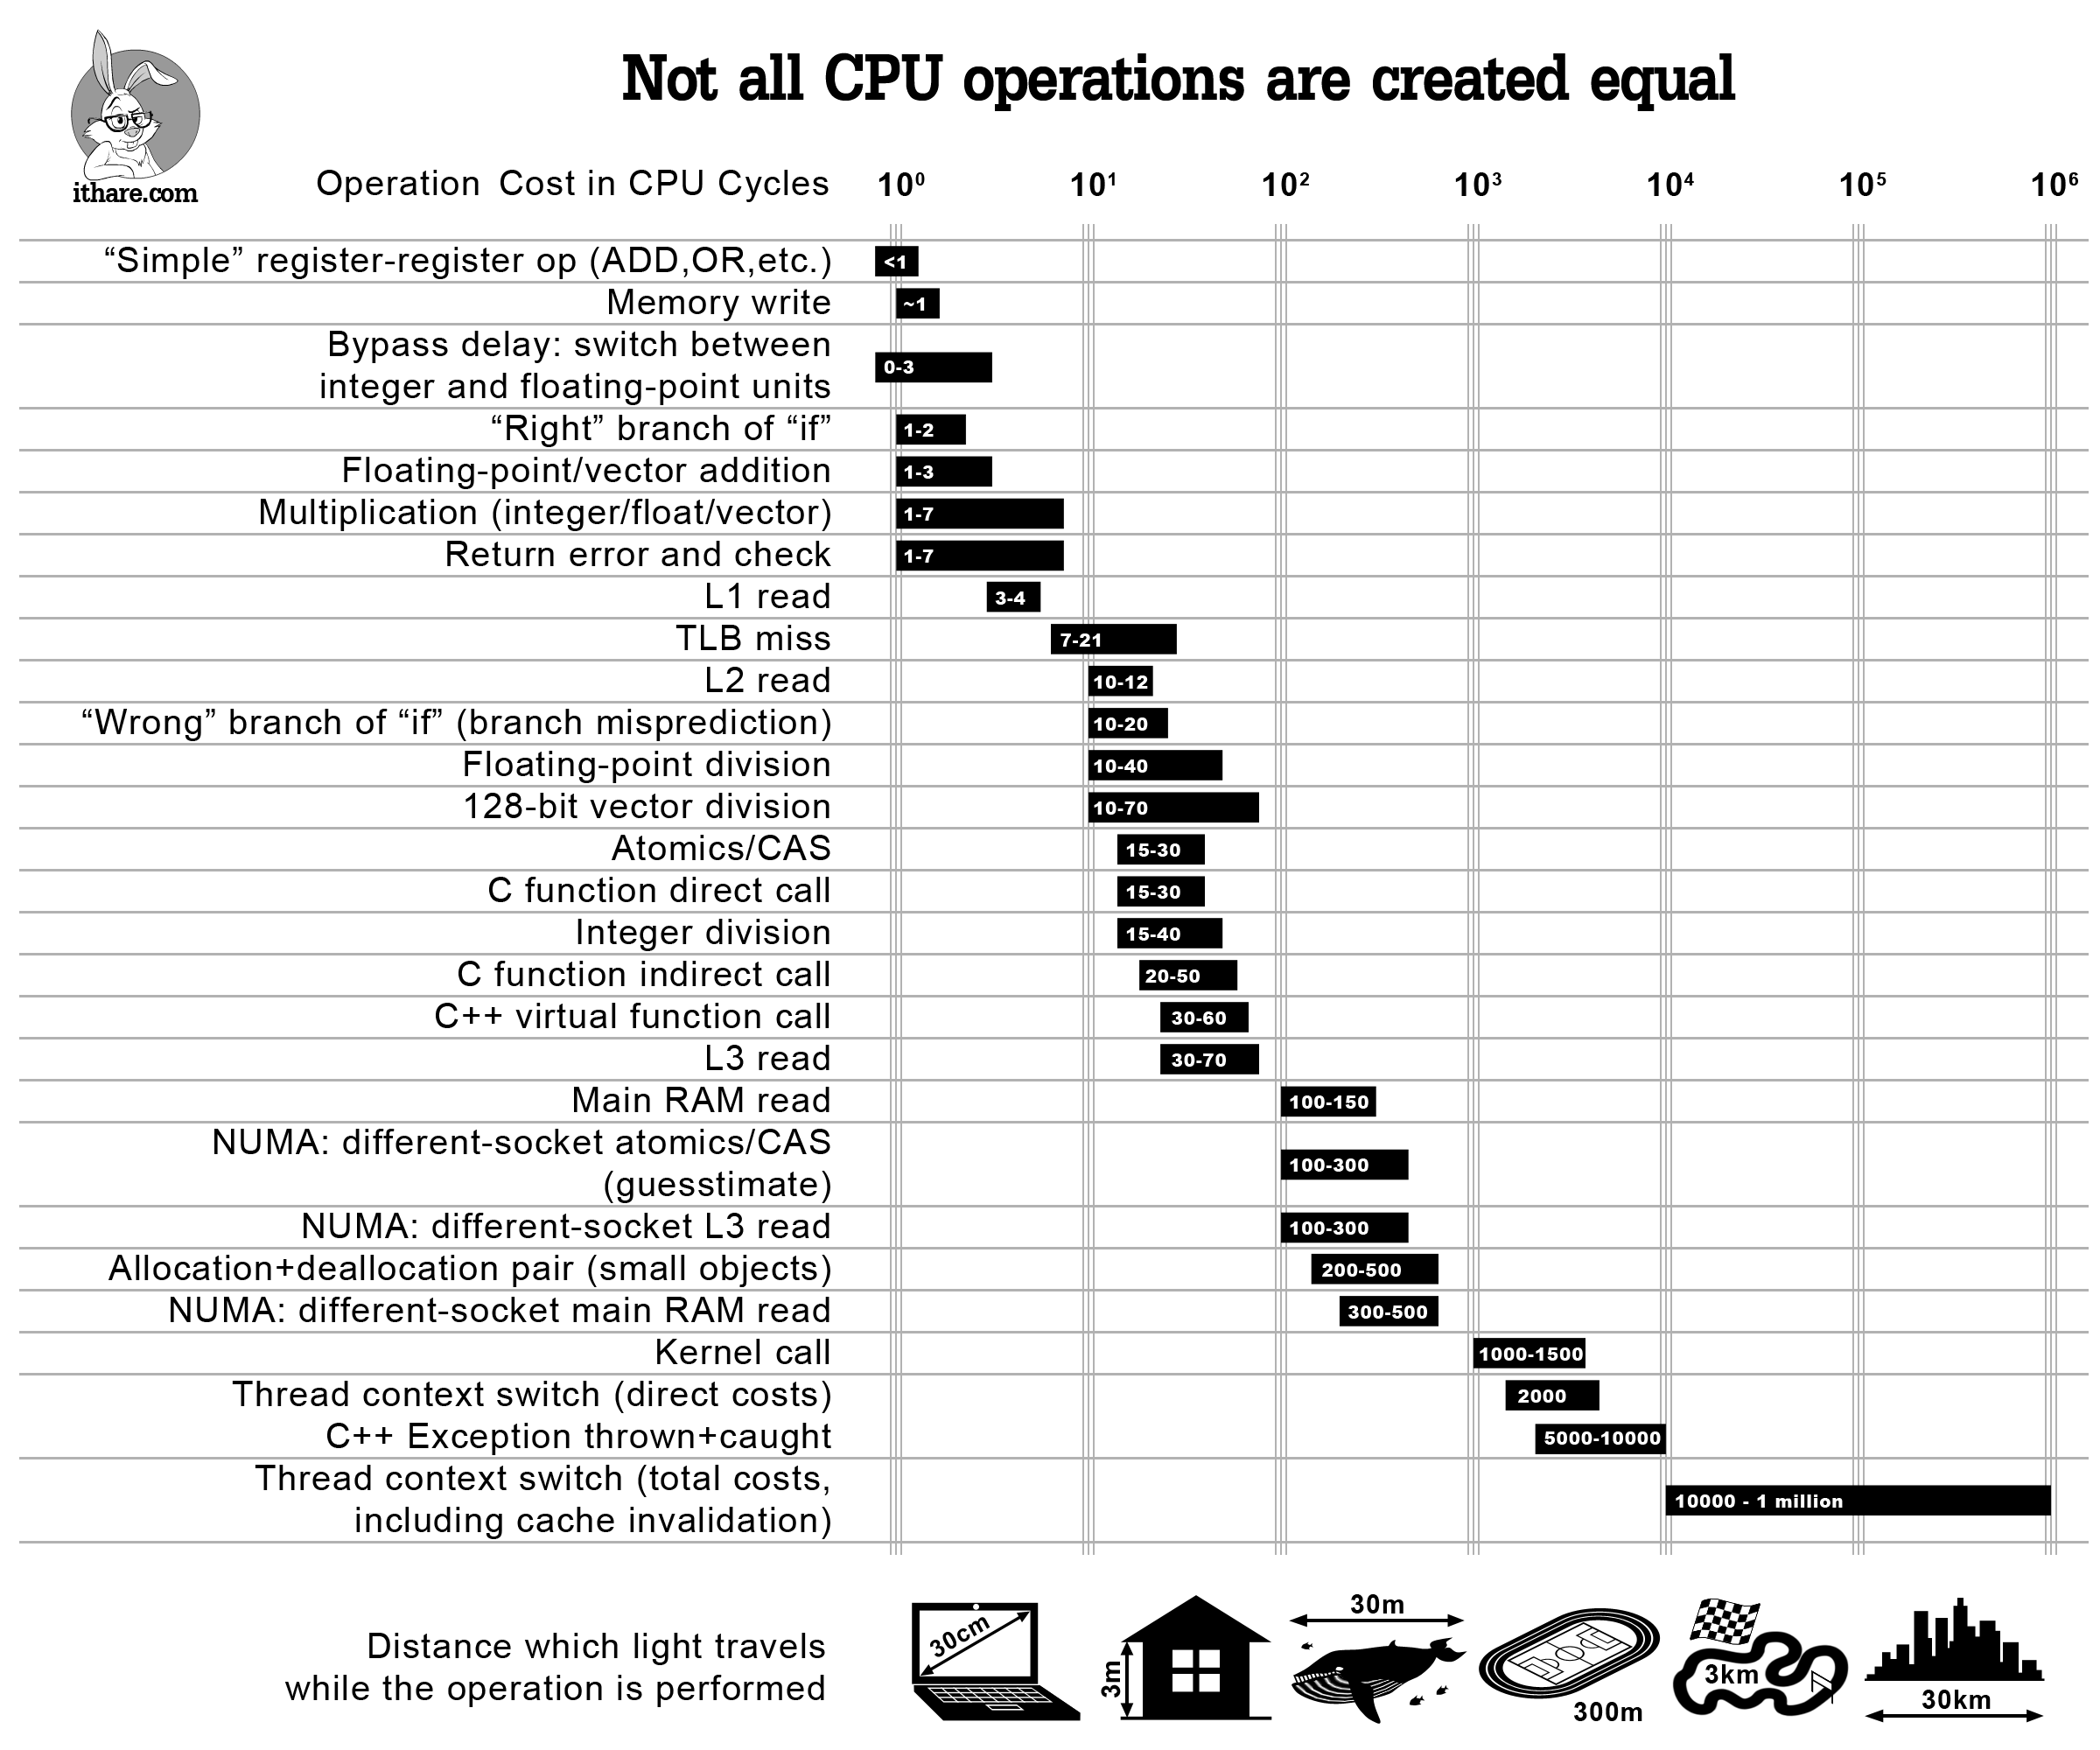
\includegraphics[width=\textwidth]{part101_infographics_v08}
\caption{Operation Costs in CPU Clock Cycles\cite{archcost}}
\end{figure}

For instance, for an x86 CPU, the associated rComplexity class would be
$ O_{1}(c_{noConflict} * n) $, where $c_{noConflict}$ is a constant corresponding to the no. of cycles required to perform the operations inner the for-loop.

For the pseudocode:
\begin{algorithmic}[1]
	\For {i=1..row-1}
		\If {currentMatrix[i][column] = 1}
			\State \Return FALSE
		\EndIf
	\EndFor
\end{algorithmic}
In a broad manner, we can estimate that the cost for the inner snippet is $c_{computeOffset} + c_{readMemory} + c_{check=1}$, where in order to compute offset, we need to perform $i * ROWS + column$, so
$ c_{computeOffset} = O_{1}(c_{addition} + c_{multiplication} + 3 * c_{readMemory})$.
Looking in a x86 Cycle cost table for operation, we can estimate the primitives $c_{addition} = O_{1}(4)$ and $c_{multiplication} = O_{1}(4)$. For memory access, the time varies, on reasons based on cache mechanics, prefetch and other runtime mechanism for improvement in speed of read operations. A satisfying margin would be $c_{readMemory} = O_{1}(100)$. 
Suppose for a complete check and jump in code $c_{check=1} = 10$

Therefore, for the inner snippet using the abose estimations, the rComplexity would be $O_{1}(4 * 100 + 4 + 4 + 10) = O_{1}(418)$. Now, the whole snippet will have the complexity $O_{1}((418 + c_{for\_checks}) \cdot n)$, where  $c_{for\_checks} = c_{check=row} + c_{addition}$ is the associated cost for incrementing the index and other checks. Thus, the rComplexity of the snippet is $O_{1}((418 + 14) \cdot n) = O_{1}(432 \cdot n)$ using the abose estimations.

 
For an exact value, we need to check the associated generated assembly code for the architecture (example x86-32bit):
\begin{verbatim}
f:
        push    ebp
        mov     ebp, esp
        sub     esp, 16
        mov     DWORD PTR [ebp-4], 0
        jmp     .L2
.L5:
        mov     eax, DWORD PTR [ebp-4]
        imul    edx, eax, 400
        mov     eax, DWORD PTR [ebp+16]
        add     edx, eax
        mov     eax, DWORD PTR [ebp+12]
        mov     eax, DWORD PTR [edx+eax*4]
        cmp     eax, 1
        je      .L6
        add     DWORD PTR [ebp-4], 1
.L2:
        mov     eax, DWORD PTR [ebp-4]
        cmp     eax, DWORD PTR [ebp+8]
        jl      .L5
        jmp     .L1
.L6:
        nop
.L1:
        leave
        ret  
\end{verbatim}


The inner loop calculus are provided inner $.L5$ label. Having this code and the x86 cycles/instructions table, we can calculate the ideal rComplexity $\Theta_{1}(n \cdot (c_{.L2} + c_{.L5}))$. Also, $c_{.L2} = c_{mov} + c_{cmp} + c_{li}$ and $c_{.L5} = c_{mov} + c_{imul} + c_{mov} +  c_{add} + c_{mov} + c_{mov} + c_{cmp} + c_{je} + c_{add} $. Using reflexivity, we conclude the rComplexity of the snippet 1 is \[f_{snippet_{1}} =  \Theta_{1}(n \cdot ( 5 * c_{mov} + c_{imul} + 2 * c_{add} +2 *  c_{cmp} + c_{je} + c_{li}))\]

Having this snippet's associated complexity calculated, we can proceed to calculate the other independent for-loops in the noConflict function:
\begin{algorithmic}[1]
	\For {j=column..n}
	\If {currentMatrix[i][j] = 1}
			\State \Return FALSE
		\EndIf
	\If {$i \leq 0$}
		\State break
	\EndIf
	\State $i \gets i-1$	
	\EndFor
\end{algorithmic}
We will associate the complexity function of this snippet with $f_{snippet_{2}}$. Similarly, for the snippet:

\begin{algorithmic}[1]
	\For {j=column..0 : increment -1}
	\If {currentMatrix[i][j] = 1}
			\State \Return FALSE
		\EndIf
	\If {$i \leq 0$}
		\State break
	\EndIf
	\State $i \gets i-1$	
	\EndFor
\end{algorithmic}
a complexity function will be obtained described by $f_{snippet_{3}}$.

Using addition properties, the complexity function for the procedute noConflict will be $f_{snippet_{1}} + f_{snippet_{2}} + f_{snippet_{3}} = O_{1}(c_{noConflict} \cdot n)$., where $c_{noConflict} \cdot n$ is the architecture-dependant constant. For instance, for x86, we can approximate $c_{noConflict \cdot n} = 432 * 3 = 1296$ and $f_{snippet_{1}} + f_{snippet_{2}} + f_{snippet_{3}} = O_{1}(1296 \cdot n) $.



Going deeper tracing the flow, we can evaluate the complexity of QueenProblem procedure by checking all elements involved in the procedure.
 \[QueenProblem(n) = O_{1}(recursiveCall) + O_{1}(noConflict) + O_{1}(overhead) + O_{1}(basecaseComplexity) \]
 \[QueenProblem(n) = n \cdot QueenProblem(n-1) +  O_{1}(1296 \cdot n) (c_{overheadFor} + c_{setBitsMatrix}) \cdot O_{1}(n) \]
 \[ QueenProblem_{1}(1)=O_{1}(c_{printMatrix})\]
 where $O_{1}(1296 \cdot n)$ is the rComplexity for the noConflict check.
 
Using the previous estimation, we assume $c_{overheadFor} = 14$ and $c_{setBitsMatrix} = 108$. Thus, the recurrent equation looks as follows: 
\[QueenProblem(n) = n \cdot QueenProblem(n-1) +  O_{1}(1418 \cdot n) \]

For the base case, we need to find the complexity of printMatrix method.
\[ QueenProblem(1)=O_{1}(n^{2} \cdot  (c_{computeOffset} + c_{readMatrixElement}))\]
\[ QueenProblem(1)=O_{1}(n^{2} \cdot  408) \]

For simplicity, we can rewrite:
\[QueenProblem(n) = n \cdot QueenProblem(n-1) +  1418 \cdot O_{1}(n) \]
\[ QueenProblem(1)= 408 \cdot O_{1}(n^{2}) \]

We can model the system as an recurrence equation:
\[ g(n) = n \cdot  g(n-1) + 1418 \cdot  n; g(0) = 408 \cdot  n^{2} \]
with the solution:
\[ 408 \cdot n^{3} \Gamma(n) + 1418 \cdot e \cdot  n \cdot \Gamma(n, 1)\]
where $\Gamma$ represents the gamma function that satisfies \[ \Gamma \left( x \right) = \int\limits_0^\infty {s^{x - 1} e^{ - s} ds} \] and $ \Gamma(n,x)$ represents the incomplete gamma function that satisfies \[ \Gamma \left(x, n \right) = \int\limits_n^\infty {s^{x - 1} e^{ - s} ds}\]

The solution of this recurrence equation in rComplexity calculus (with $n \in \mathbb{N}$) is:
\[ QueenProblem(n) = O_{1}(408 \cdot n^{2} \cdot n!) +  O_{1}(1418 \cdot n \cdot n!) \]
Using the $O_{1}$ addition properties, we conclude:
\[ QueenProblem(n) = O_{1}(408 \cdot n^{2} \cdot n!) \]